\section{Zielsetzung}
In diesem Versuch sollen die Schwingungs-und Schwebungsdauern von
gekoppelten Pendeln bei gleichphasiger, gegenphasiger und gekoppelter
Schwingung gemessen werden.
\section{Theorie}
\label{sec:Theorie}
Im Folgenden wird ein Pendel mit Masse $m$ und der Fadenlänge $l$
betrachtet. Auf Dieses wirkt bei Auslenkung die Gewichtkraft $\vec{F} = m\vec{g}$
und das Drehmoment $ M = D_p \phi $, dabei ist $\phi$ der Auslenkungswinkel
und $D_p$ die Winkelrichtgröße. Zudem gilt für kleine Winkel $\symup{sin}\phi
\approx \phi$. Die Bewegungsgleichung für so ein Pendel lautet dann
\begin{equation*}
  J \ddot{\phi} + D_p \phi = 0\, ,
\end{equation*}
dabei ist $J$ das Trägheitsmoment des Pendels. Die Lösung dieser Bewegungsgleichung
ist dann für eine harmonische Schwingung die Schwingungsfrequenz
\begin{equation}
  \omega = \sqrt{\frac{D_p}{J}} = \sqrt{\frac{g}{l}}\;.
  \label{eqn:l1}
\end{equation}
Werden zwei mit einer Feder gekoppelte Pendel betrachtet,
erhält jedes Pendel eine Bewegungsgleichung
mit einem zusätzlichen Drehmoment $D_F$ . Somit ergeben sich die gekoppelten
Differentialgleichungen
\begin{equation*}
J \ddot{\phi_1} + D_p \phi_1 = D_F( \phi_2 - \phi_1) \quad \text{und} \quad
J \ddot{\phi_2} + D_p \phi_2 = D_F( \phi_1 - \phi_2)\;.
\end{equation*}
Durch eine geschickte Wahl der Winkel lässt sich dieses
Differentialgleichungssystem entkoppeln und lösen. Die Lösung hängt dabei von
den Anfangsbedingungen $\alpha(t=0)$ und $\dot{\alpha}(t=0)$ ab. Dabei bezeichnen
$\alpha_1$ und $\alpha_2$ die Auslenkungswinkel (siehe Abb. \ref{fig:pendel}).

\begin{figure}
  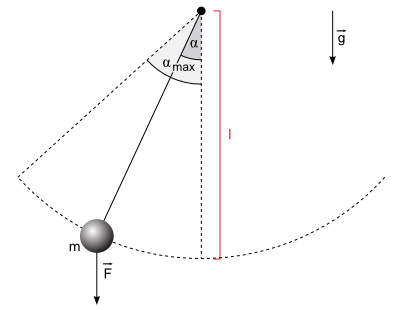
\includegraphics[width = \textwidth]{./logos/5222.png}
  \caption{Skizze zur Winkeldefinition.\cite{Skizze}}
  \label{fig:pendel}
\end{figure}

Die Lösungen können dann wie im Folgenden dargestellt werden.
\begin{itemize}
  \item Bei \textbf{gleichphasiger Schwingung} gilt $\alpha_1 = \alpha_2$ .
  Daraus ergibt sich dann für die Schwingungsfrequenz $\omega_+$
  und die Schwingungsdauer $T_+$
  \begin{equation}
  \omega_+ = \sqrt{\frac{g}{l}} \quad \text{und} \quad
  T_+ = 2\pi \sqrt{\frac{l}{g}}\;.
  \label{eqn:gls}
\end{equation}
\item Bei der \textbf{gegenphasigen Schwingung} gilt $\alpha_1 = - \alpha_2$,
daraus ergeben sich
\begin{equation}
   \omega_- = \sqrt{\frac{g}{l} + \frac{2K}{l}} \quad \text{und} \quad
   T_- = 2\pi \sqrt{\frac{l}{g+2K}}\;.
   \label{eqn:ggs}
 \end{equation}
 Hierbei bezeichnet $K$ die Kopplungskonstante der Feder zwischen den Pendeln.
 \item Bei der \textbf{gekoppelten Schwingung} gilt $\alpha_1 = 0, \alpha_2 \neq 0$,
 dann ergibt sich
 \begin{equation}
   \omega_S = \omega_+ - \omega_- \quad \text{und} \quad
   T_S = \frac{T_+\cdot T_-}{T_+ - T_-}\;,
   \label{eqn:gks}
 \end{equation}
 dabei bezeichnet $\omega_S$ die Schwebungsfrequenz und $T_S$ die Schwebungsdauer.
 Die Kopplungskonstante $\kappa$ wird hier mit
 \begin{equation}
   \kappa = \frac{\omega_- ^2 - \omega_+ ^2}{\omega_- ^2 + \omega_+ ^2}
   = \frac{T_+ ^2 - T_- ^2}{T_+ ^2 + T_- ^2}
   \label{eqn:K}
 \end{equation}
 definiert.

 \end{itemize}
